\chapter{ナノフォトニック・デバイスを用いたRace Logic実装の提案}
本章では,本提案のナノフォトニック・デバイスを用いたRace Logic(以下,光Race Logic)回路を理解する上で必要な光デバイスに関する基本事項を説明し,光Race Logic実装について述べる.

\section{光デバイスについて}
本節では,まず光デバイスの特徴と代表的な光素子,ナノフォトニクスについて説明する.
その後,光デバイスとRace Logicの親和性について述べる.

\subsection{光デバイスの特徴}
以下に光デバイスの特徴をまとめ,詳細を説明する.
光デバイスは光が信号を伝搬する素子全般のことを指す.
一方,本論文では電気デバイスとは電気が信号を伝搬するCMOSトランジスタを指すものと定義する.
\begin{itemize}
\item デバイスサイズ\\
現状,光デバイスのゲート長は$cm$〜$mm$オーダーのスケールである.後述するナノフォトニクスを用いたとしても,そのスケールのオーダーは$\mu m$である.
\item 信号の周波数帯域\\
光デバイスにおいて,信号の伝搬は光信号が通過するか否かで行われる.電気デバイスのように時定数によって周波数帯域が制限されることがない.よって,その周波数帯域は広帯域であると言える.
\item データの蓄積\\
電気デバイスは,電荷を貯めることでデータを保持できる.光デバイスは光を留めておくことが難しいため,データの蓄積は困難である.電気デバイスの方が,光デバイスよりもデータの蓄積が容易であると言える.
\item スループット\\
データ処理やネットワークにおいてのスループットについて述べる.
スループットとは単位時間あたりの処理量や処理可能なデータ量のことである.
光信号は多重性と呼ばれる複数の異なる周波数を多重して送る事ができる性質を持つ.
光デバイスは光信号の広帯域性や,波長多重,位相多重と言った多重性を利用して,
伝搬信号自体の情報量を増加させることで,データ転送速度を向上させることが可能である.
\end{itemize}

電気デバイスはデバイスの小型化が可能という特徴から集積度を上げることが可能である.
それに比べ,現状では光デバイスはデバイスの小型化に向いておらず,集積度を上げることが困難であった.
よって演算には電気デバイスが用いられてきた.
一方,光デバイスは伝搬信号の情報量が大きく,信号の移動速度も速いという特徴から通信に使われてきた.

\subsection{光素子の説明}
本項では,代表的な光素子について説明する.その説明にあたり,語句を定義する.
\begin{itemize}
\item 光伝搬信号\\
光デバイスおよび,そのデバイスを用いて構成した回路において,情報を伝搬する光信号を指す.
\item 光伝搬入力信号および光伝搬出力信号\\
光デバイスおよび,そのデバイスを用いて構成した回路において,入力される光伝搬信号を光伝搬入力信号,出力される光伝搬信号を光伝搬出力信号と呼ぶ.光入力信号および光出力信号と略す.
\item 光伝搬入力信号強度および光伝搬出力信号強度\\
光伝搬入力信号および光伝搬出力信号の信号強度を指す.単位は[W]である.光入力信号強度および光出力信号強度と略す.
\item 光制御信号\\
光デバイスを制御するための光信号を指す.
\item 光制御信号強度\\
光制御信号の信号強度を指す.単位は[W]である.
\item 電気制御信号\\
光デバイスを制御するための電気信号を指す.
\item 電気制御信号強度\\
電気制御信号の信号強度を指す.単位は[V]である.
\end{itemize}

\subsubsection{光スイッチ}
光スイッチとは,光伝搬信号を通過させるか否かでオン動作およびオフ動作をする光デバイスである.
光スイッチの性能指標として,よく用いられるのが漏れ率および透過率,消光比である.
\begin{figure}[t!]
\begin{center}
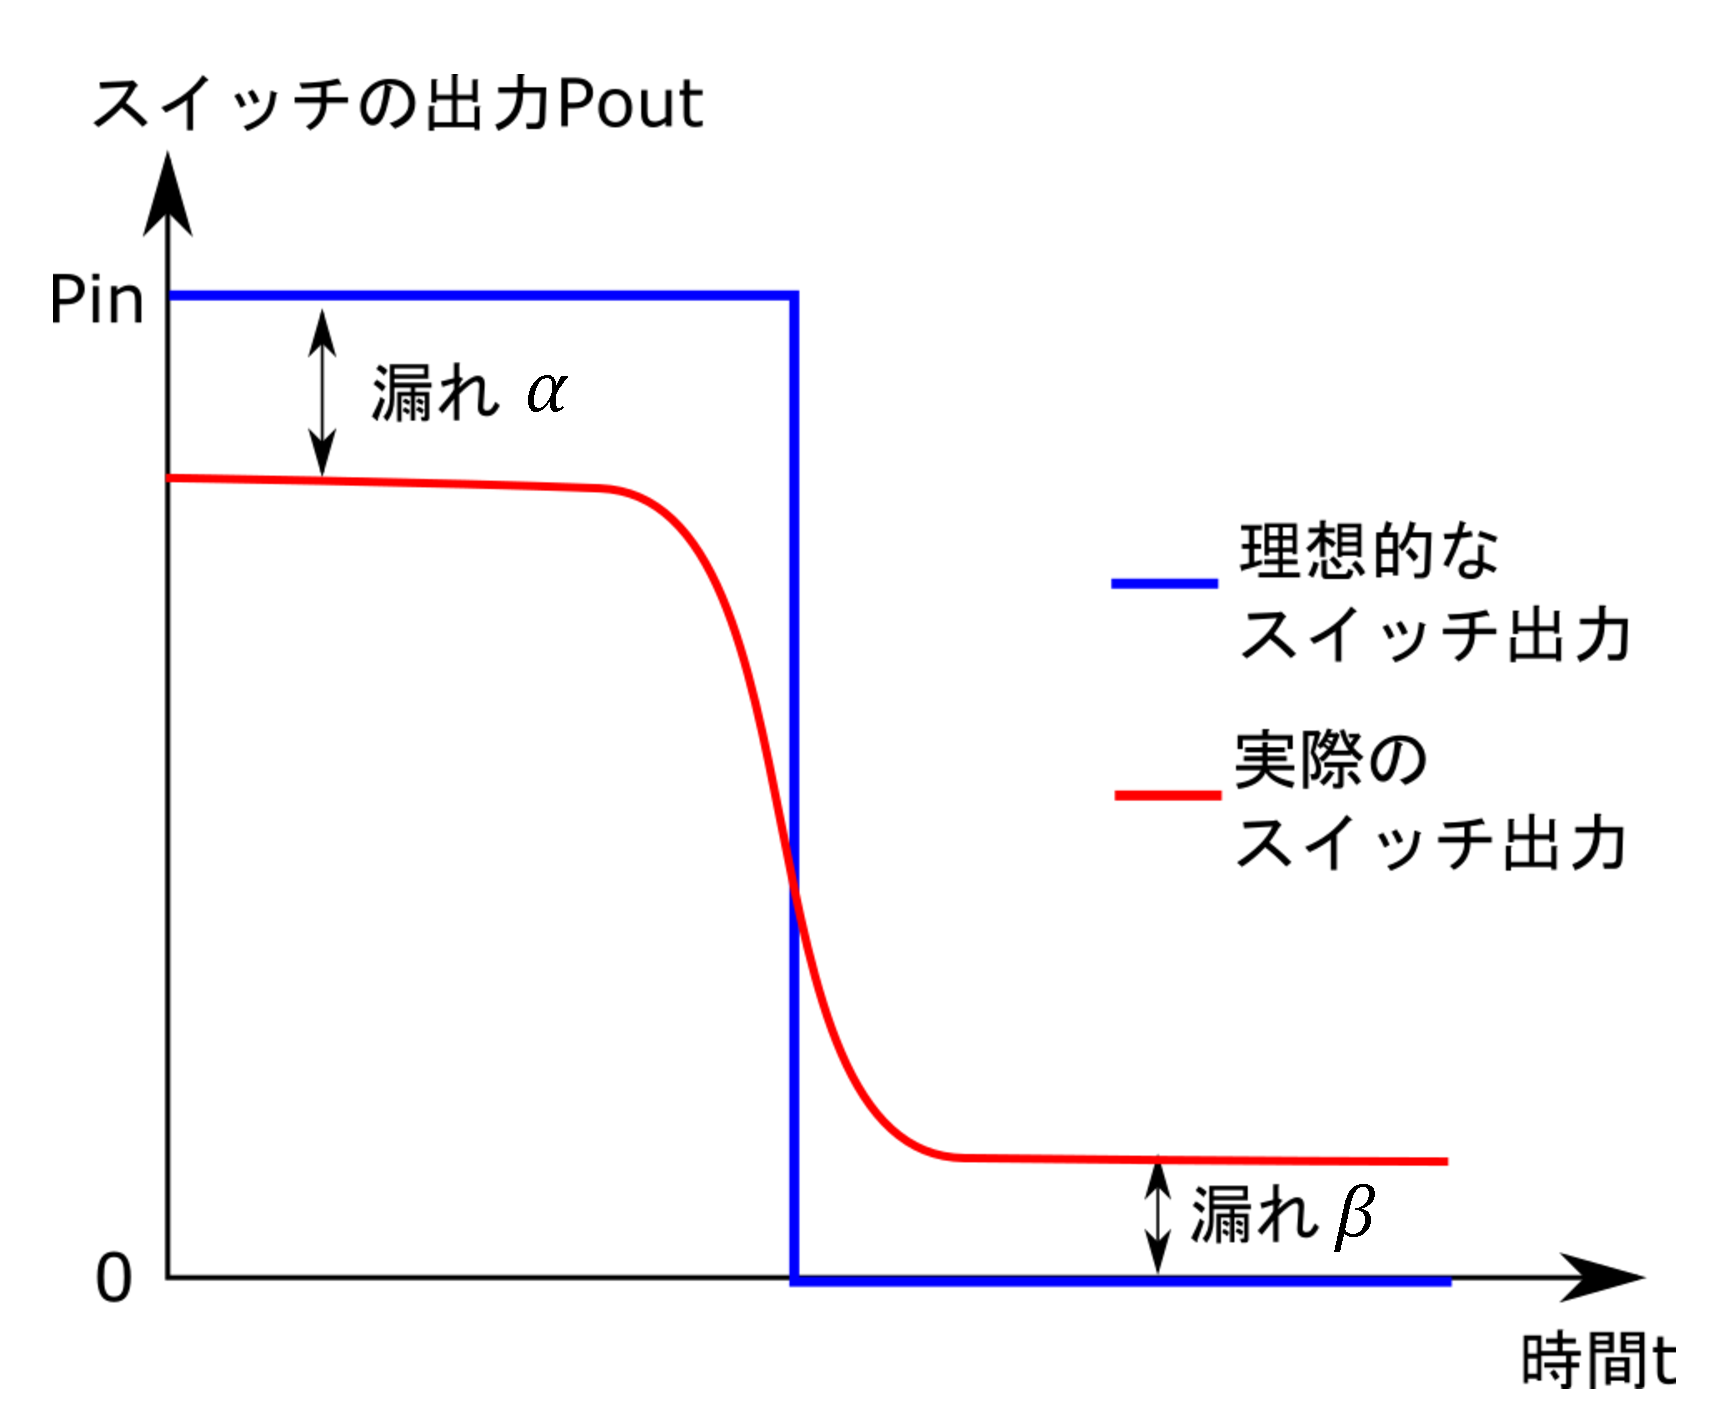
\includegraphics[keepaspectratio,scale=0.25]{fig/3/swichout.pdf}
\caption{光スイッチの光入力信号強度と光出力信号強度}
\label{fig:swichout}
\end{center}
\end{figure}
光スイッチへの光入力信号強度を$P_{in}$,光出力信号強度を$P_{out}$とした場合の,
光入力信号強度と光出力信号強度の関係を図 \ref{fig:swichout}に示す.
図の縦軸は光出力信号強度,横軸は時間を表している.
理想的なスイッチでは,光伝搬信号の漏れが無いため光出力信号強度は図の青線に示す関係を取る.
しかしながら,実際にはオン動作とオフ動作どちらの場合でも光伝搬信号の漏れがあるため,
光出力信号強度は図の赤線に示す関係を取る.以下にそれぞれの性能指標の定義を示す.
\begin{itemize}
\item 漏れ率,透過率\\
漏れ率とは,スイッチがオン動作とオフ動作の際,
それぞれどの程度の光伝搬信号が漏れるかということを表す指標である.
図 \ref{fig:swichout}に示す$\alpha $は,
スイッチがオン動作の際にスイッチから回路外へ光伝搬信号がどの程度漏れ出すかを表す漏れ率である.
また,スイッチがオン動作の際にどの程度の光伝搬信号を透過させられるかを表す指標を透過率と呼び,
漏れ率$\alpha$を用いて表すと$1- \alpha$となる.
光スイッチへの光入力信号強度を$P_{in}$,オン動作をする際の光出力信号強度を
$P_{1out}$とすると,$\frac{P_{1out}}{P_{in}}=1- \alpha$である.
図 \ref{fig:swichout}に示す$\beta $は,スイッチがオフ動作の際に光伝搬信号を遮断しきれずに,
どの程度出力へ漏れ出すかを表す漏れ率である.
光スイッチへの光入力信号強度を$P_{in}$,
オフ動作をする際の光出力信号強度を$P_{0out}$とすると,
$\frac{P_{0out}}{P_{in}}=\beta$である.
$\alpha $,$ \beta $の値が小さいほどスイッチの性能が高いと言える.
\item 消光比\\
消光比とは,スイッチの光出力信号が1と0の場合の光出力信号強度比である.
透過率$1- \alpha$および漏れ率$\beta $用いると,
式~\eqref{eq:syoukouhi}で表される.
\begin{equation}
消光比= \frac{1- \alpha}{\beta}
\label{eq:syoukouhi}
\end{equation}
\end{itemize}
%式~\eqref{eq:syoukouhi}および式~\eqref{eq:oma}から,

消光比は,透過率および漏れ率を用いて議論することが可能であるとわかる.
よって本論文では透過率,漏れ率に着目し,これらをスイッチ性能として議論する.

\subsubsection{受光器}
光の素粒子は一般に光子(フォトン)と呼ばれる.
全ての粒子が波動性を持つことを,粒子と波動の二重性と言う.
光子も粒子性と波動性の2つの性質を持つ\cite{大津}.
光子のエネルギーは光の周波数(波長)で決定する.
\begin{equation}
E = h \nu \label{eq:hikarienergy}
\end{equation}
Eは光子のエネルギー,hはプランク定数,$\nu$は光の周波数である.
光の強度は光子の数によって決定する.

物質中の電子のエネルギーは,取り得るエネルギー準位が限定されている.
そのエネルギー準位は帯構造を取り,図\ref{fig:eg}に示すようにそれぞれ伝導帯,禁制帯,価電子帯と呼ばれる.
伝導帯とは,電子が占めているエネルギー帯のうち最も高いエネルギー準位を示すエネルギー帯である.
この伝導帯は電子が充填されておらず,このエネルギー帯に存在する電子は自由電子として振る舞う.
価電子帯は価電子によって充填されたエネルギー帯である.禁制帯とは電子が存在できないエネルギー帯である.
この禁制帯の幅が図\ref{fig:eg}に示すEgであり,エネルギーギャップと呼ばれる.
半導体物質において,エネルギーギャップを超えるのに十分なエネルギーを持った光子1つが入射した際に,自由電子と正孔のペア1つを生成する.
この現象を{\bf 吸収}という.光子のエネルギーはその光の周波数で決まるため,エネルギーギャップの大きさに対応した周波数がある.
逆の現象が,{\bf 放出}である.これは,自由電子と正孔が再結合した際に,そのエネルギーギャップ$Eg=h \nu$に相当するエネルギーを持つ光子を放出する現象である.
図\ref{fig:kyusyuhosya}に吸収と放出の様子を示す.
図\ref{fig:kyusyuhosya}(a)におけるエネルギーギャップが,緑の光の光子の持つエネルギーと等しいとする.
この際,緑の光を入射すると電子正孔対が生成される.
しかしながら,赤の光は緑の光よりも周波数が小さいため,光子のエネルギーが緑の光と比べて小さい.
よって赤の光を入射しても電子は伝導帯へと励起することができず,電子正孔対は生成されない.
\begin{figure}[t!]
\begin{center}
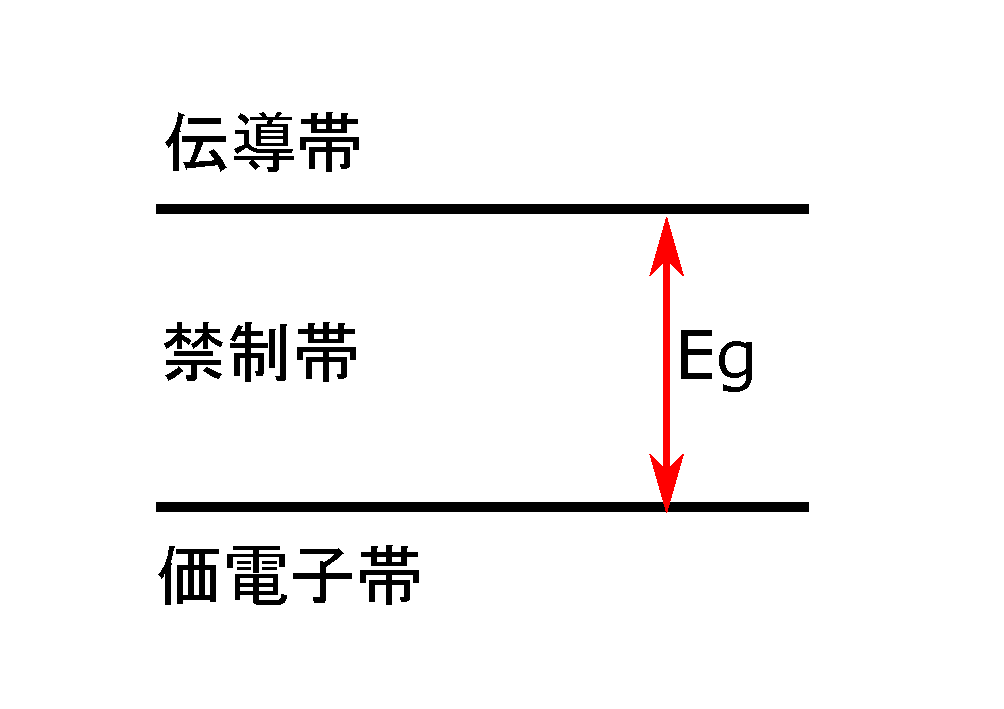
\includegraphics[keepaspectratio,scale=0.4]{fig/3/Eg.pdf}
\caption{半導体のエネルギーバンド図}
\label{fig:eg}
\end{center}
\end{figure}
\begin{figure}[t!]
\begin{center}
\subfigure[吸収]{
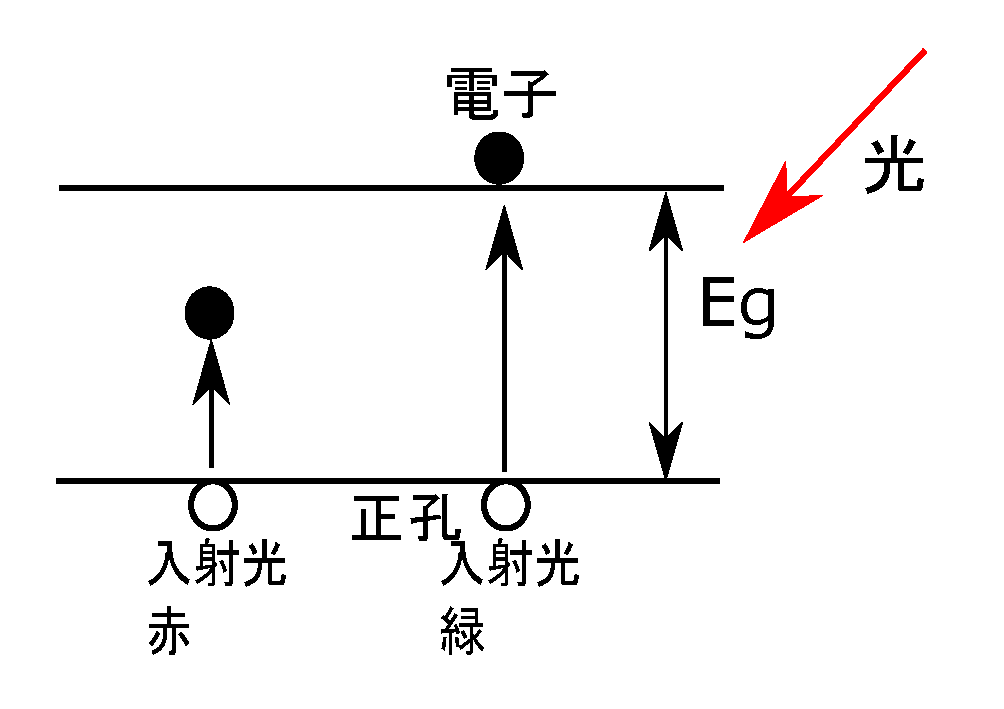
\includegraphics[keepaspectratio,scale=0.4]{fig/3/kyusyu.pdf}}
\subfigure[放出]{
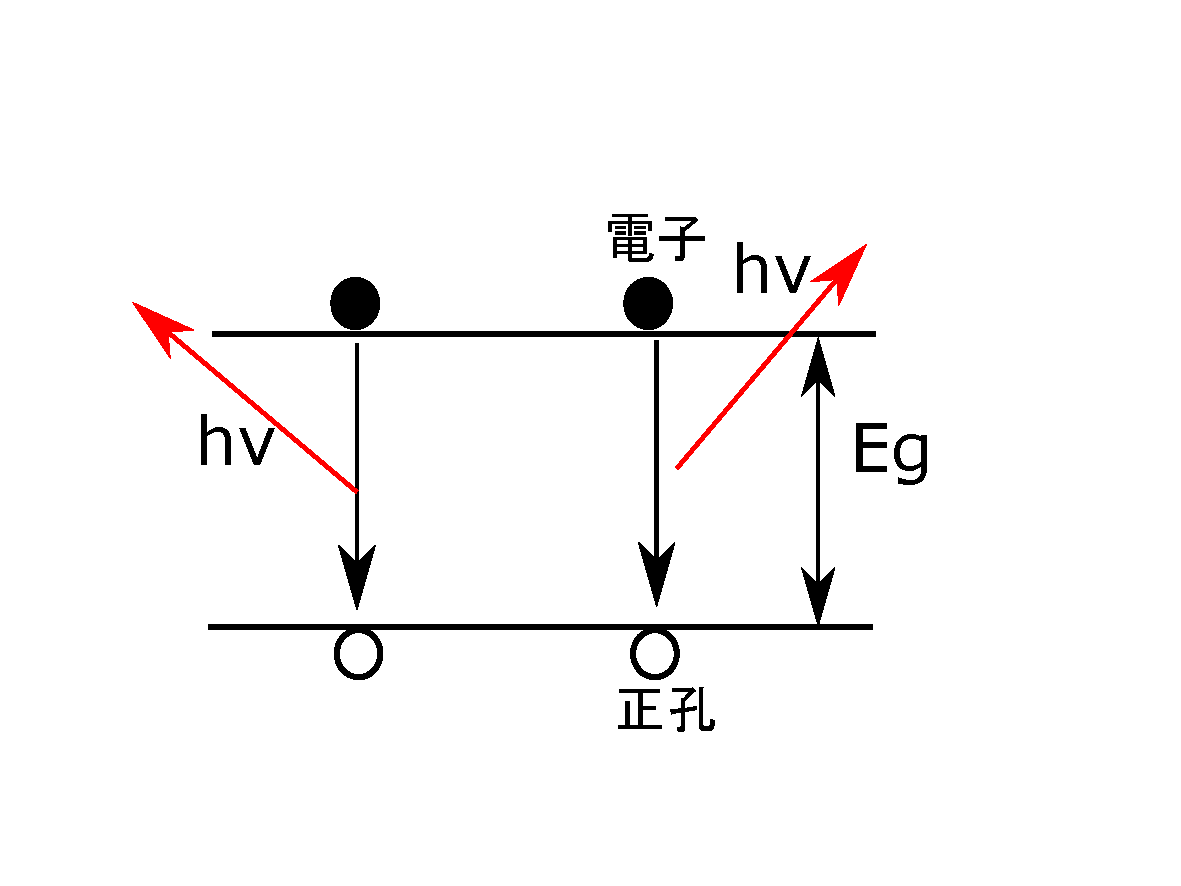
\includegraphics[keepaspectratio,scale=0.4]{fig/3/hosya.pdf}}
\caption{光の吸収と放出}
\label{fig:kyusyuhosya}
\end{center}
\end{figure}
受光器であるフォトダイオードはこの吸収の現象を利用して光を検出する.

フォトダイオードはp型半導体と真性半導体とn型半導体を接合したpin接合という構造を持ち,
空乏層で発生した電子や正孔が移動することで電流が流れる.
この電流のことを光電流と呼ぶ.
流れる光電流の大きさは光の強度に比例する.
図\ref{fig:photo}に受光器のエネルギーバンド図を示す.
\begin{figure}[t!]
\begin{center}
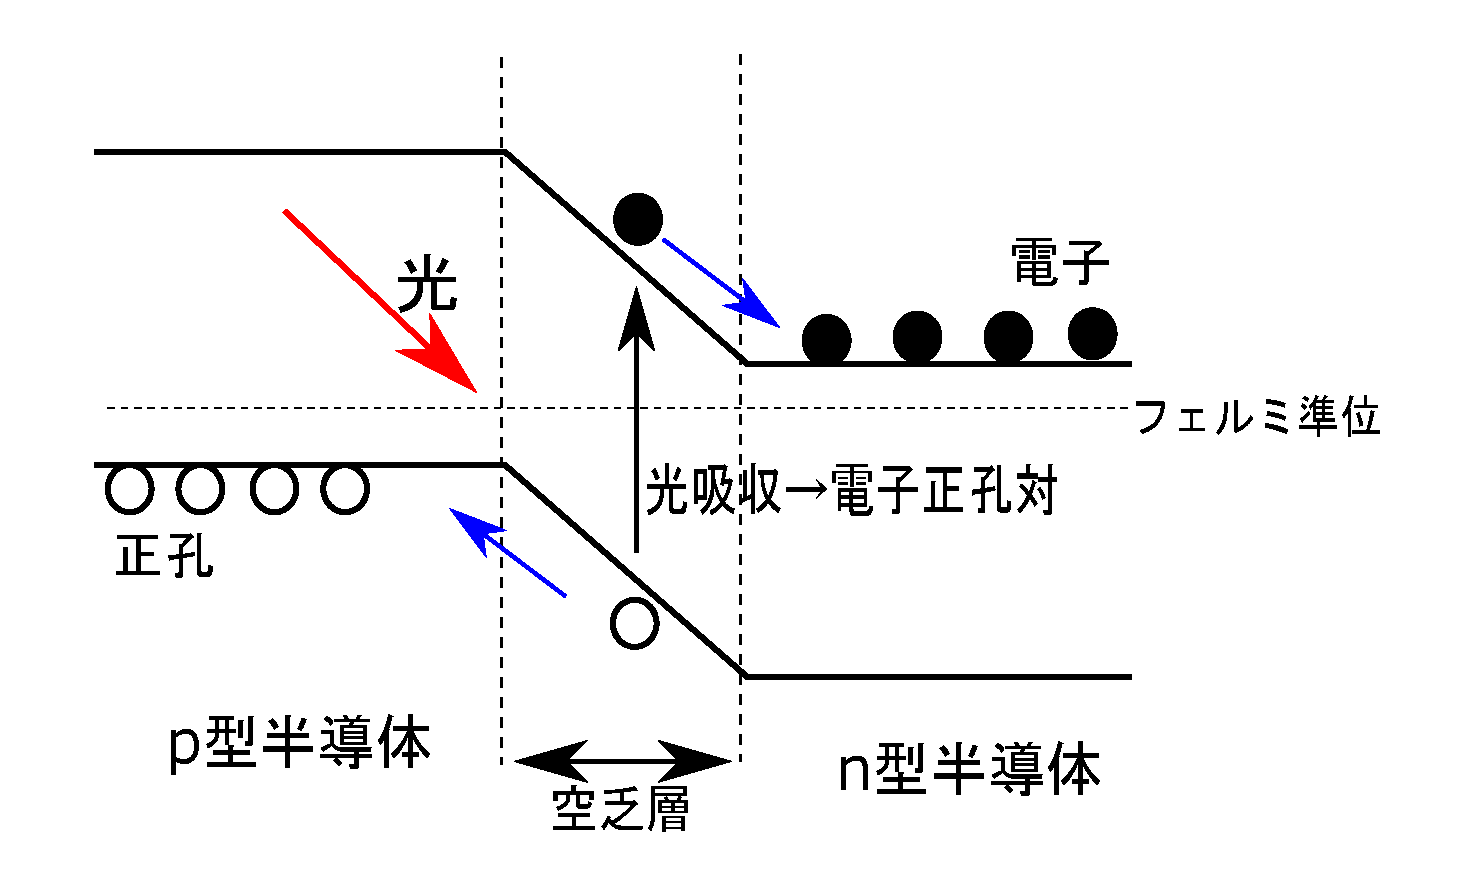
\includegraphics[keepaspectratio,scale=0.4]{fig/3/photodiode.pdf}
\caption{受光器のエネルギーバンド図}
\label{fig:photo}
\end{center}
\end{figure}

受光器の性能は受光感度として表される.
受光感度は,光入力信号強度を[W],光電流を[A]で表した場合,
両者の比で表される.
受光感度は式~\eqref{eq:jyukoukando}で表される.
式~\eqref{eq:jyukoukando} によって導かれる値が1に近い程,感度の良い受光器であることを示す.
\begin{equation}
受光感度 = \frac{A}{W}
\label{eq:jyukoukando}
\end{equation}
もう一つ重要な性能指標が受光器の最小受光感度である.最小受光感度とは,受光器が検出可能な最小の信号強度のことである.

\subsubsection{光カプラ}
光カプラとは,1つの入力端子に入射した光伝搬信号を複数の出力端子に出射する分岐・分配機能と
複数の入力端子に入射した光伝搬信号を1つの出力端子に出射する結合機能を持つデバイスである.
光分岐結合器,光分岐挿入器とも呼ばれる.
光カプラの分類を図\ref{fig:lcoup}に示す.
4端子で2入力2出力または3入力1出力のものが光方向性結合器(図\ref{fig:lcoup1}),
1入力N出力のものが光分配器もしくは光分岐器(図\ref{fig:lcoup2}),
N入力1出力のものが光結合器(図\ref{fig:lcoup3}),
N入力M出力のものが光スターカプラ(図\ref{fig:lcoup4})と呼ばれている.
光スターカプラの中には透過型と反射型という分類が存在する.
光結合器の多くが入出力端子を逆にすることで光分配器としても使うことができる\cite{ハンドブック}.
また,光の結合・分配の際には損失が発生する.
\begin{figure}[t!]
\begin{center}
\subfigure[光方向性結合器:2入力2出力]{
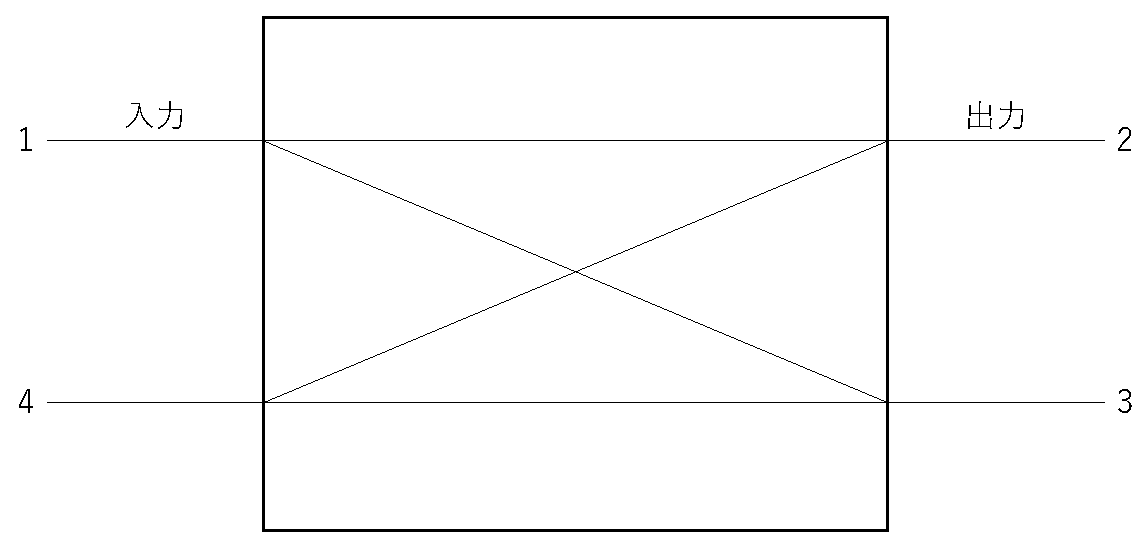
\includegraphics[keepaspectratio, scale=0.4]{fig/3/lcoup1.eps}
\label{fig:lcoup1}
}
\subfigure[光分配器:1入力N出力]{
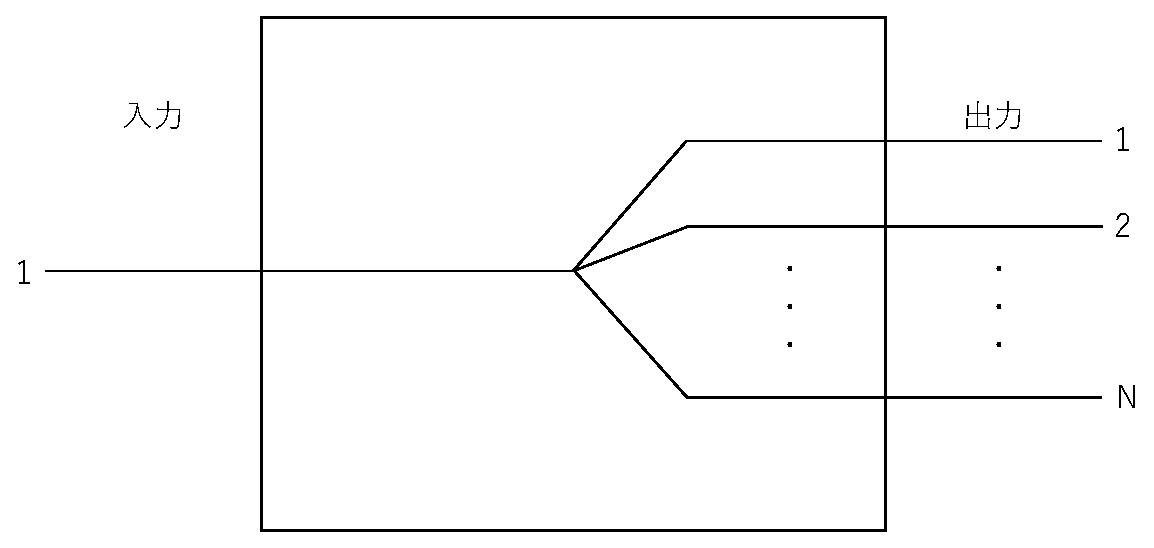
\includegraphics[keepaspectratio, scale=0.4]{fig/3/lcoup2.eps}
\label{fig:lcoup2}
}\\
\subfigure[光結合器:N入力1出力]{
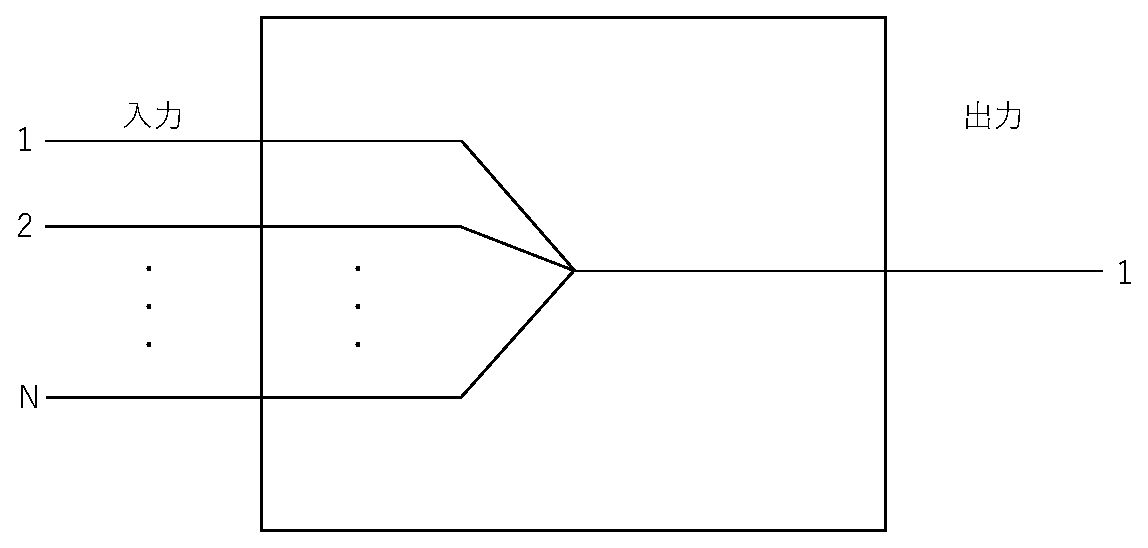
\includegraphics[keepaspectratio, scale=0.4]{fig/3/lcoup3.eps}
\label{fig:lcoup3}
}
\subfigure[光スターカプラ:N入力N出力]{
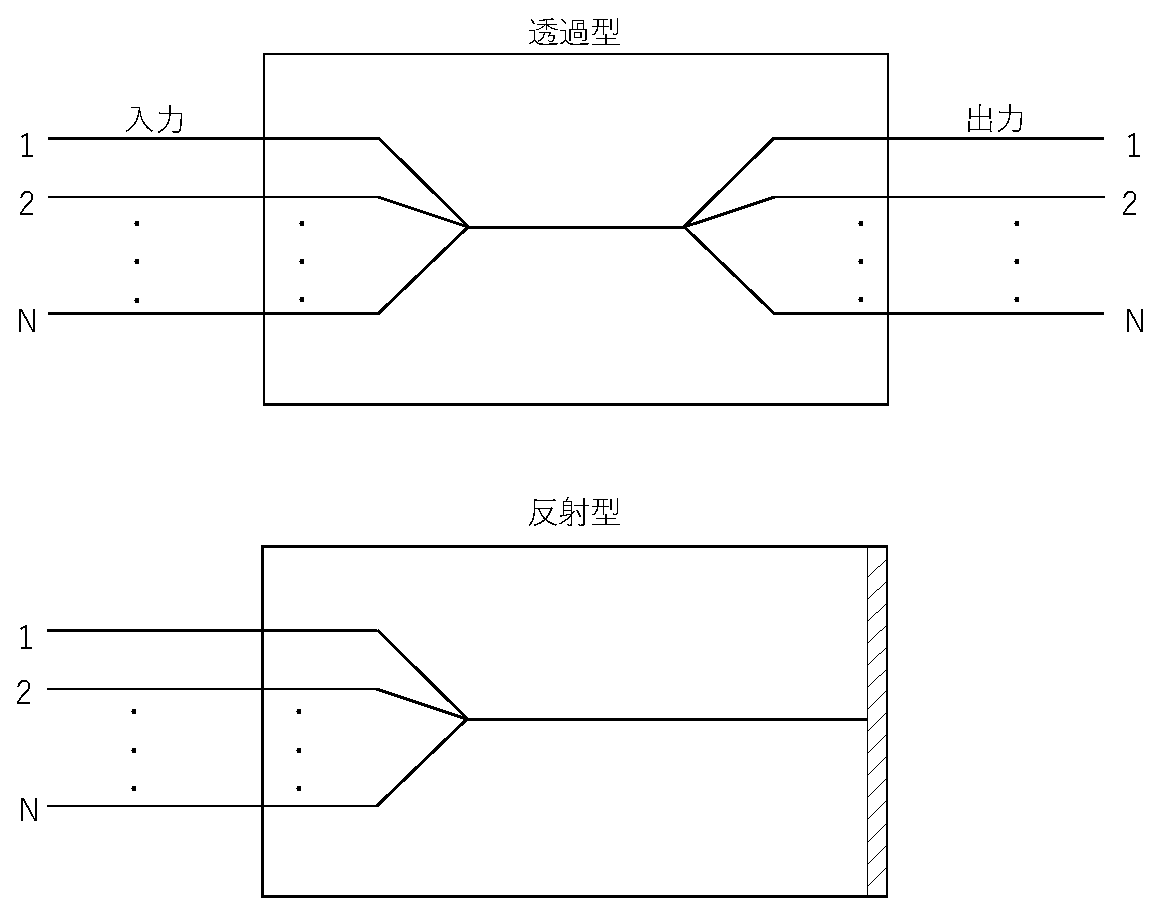
\includegraphics[keepaspectratio, scale=0.4]{fig/3/lcoup4.eps}
\label{fig:lcoup4}
}
\caption{光カプラの分類}
\label{fig:lcoup}
\end{center}
\end{figure}

\subsubsection{光遅延素子}
光遅延素子は光伝搬信号に伝搬遅延を付加できる素子のことを指す.
その実現は様々な方法があり,いずれの方法を用いても遅延を付加する際には損失が発生する.

\subsection{ナノフォトニクスの性質}
ナノフォトニクスとは,ナノ加工技術をベースとして,近接場光の性質を活かした技術である.
近接場光とは物質の表面付近に局在する非伝播な電磁場であり,その局在範囲は光の波長と同程度かそれに比べ小さい.
近接場光の概要を図\ref{fig:kinsetu}に示す.
物質から遠ざかるにつれて電磁場は減少するため,その特徴からエバネッセント光とも呼ばれる.
屈折率が大きい媒質から屈折率の小さい媒質に光を入射させる.
この場合ある角度を超えると,光は境界面を通過せず全て反射する.
この現象を全反射と言う.物質表面に全反射が起こるように光を入射した際,反射が起こっている物質境界面付近では局在する電磁場が発生する.
この電磁場光がエバネッセント光である.
エバネッセント光が発生した際,境界面から離れる方向に電磁場が弱くなる.
図\ref{fig:eva2}はエバネッセント光が発生する様子である.
\begin{figure}[t!]
\begin{center}
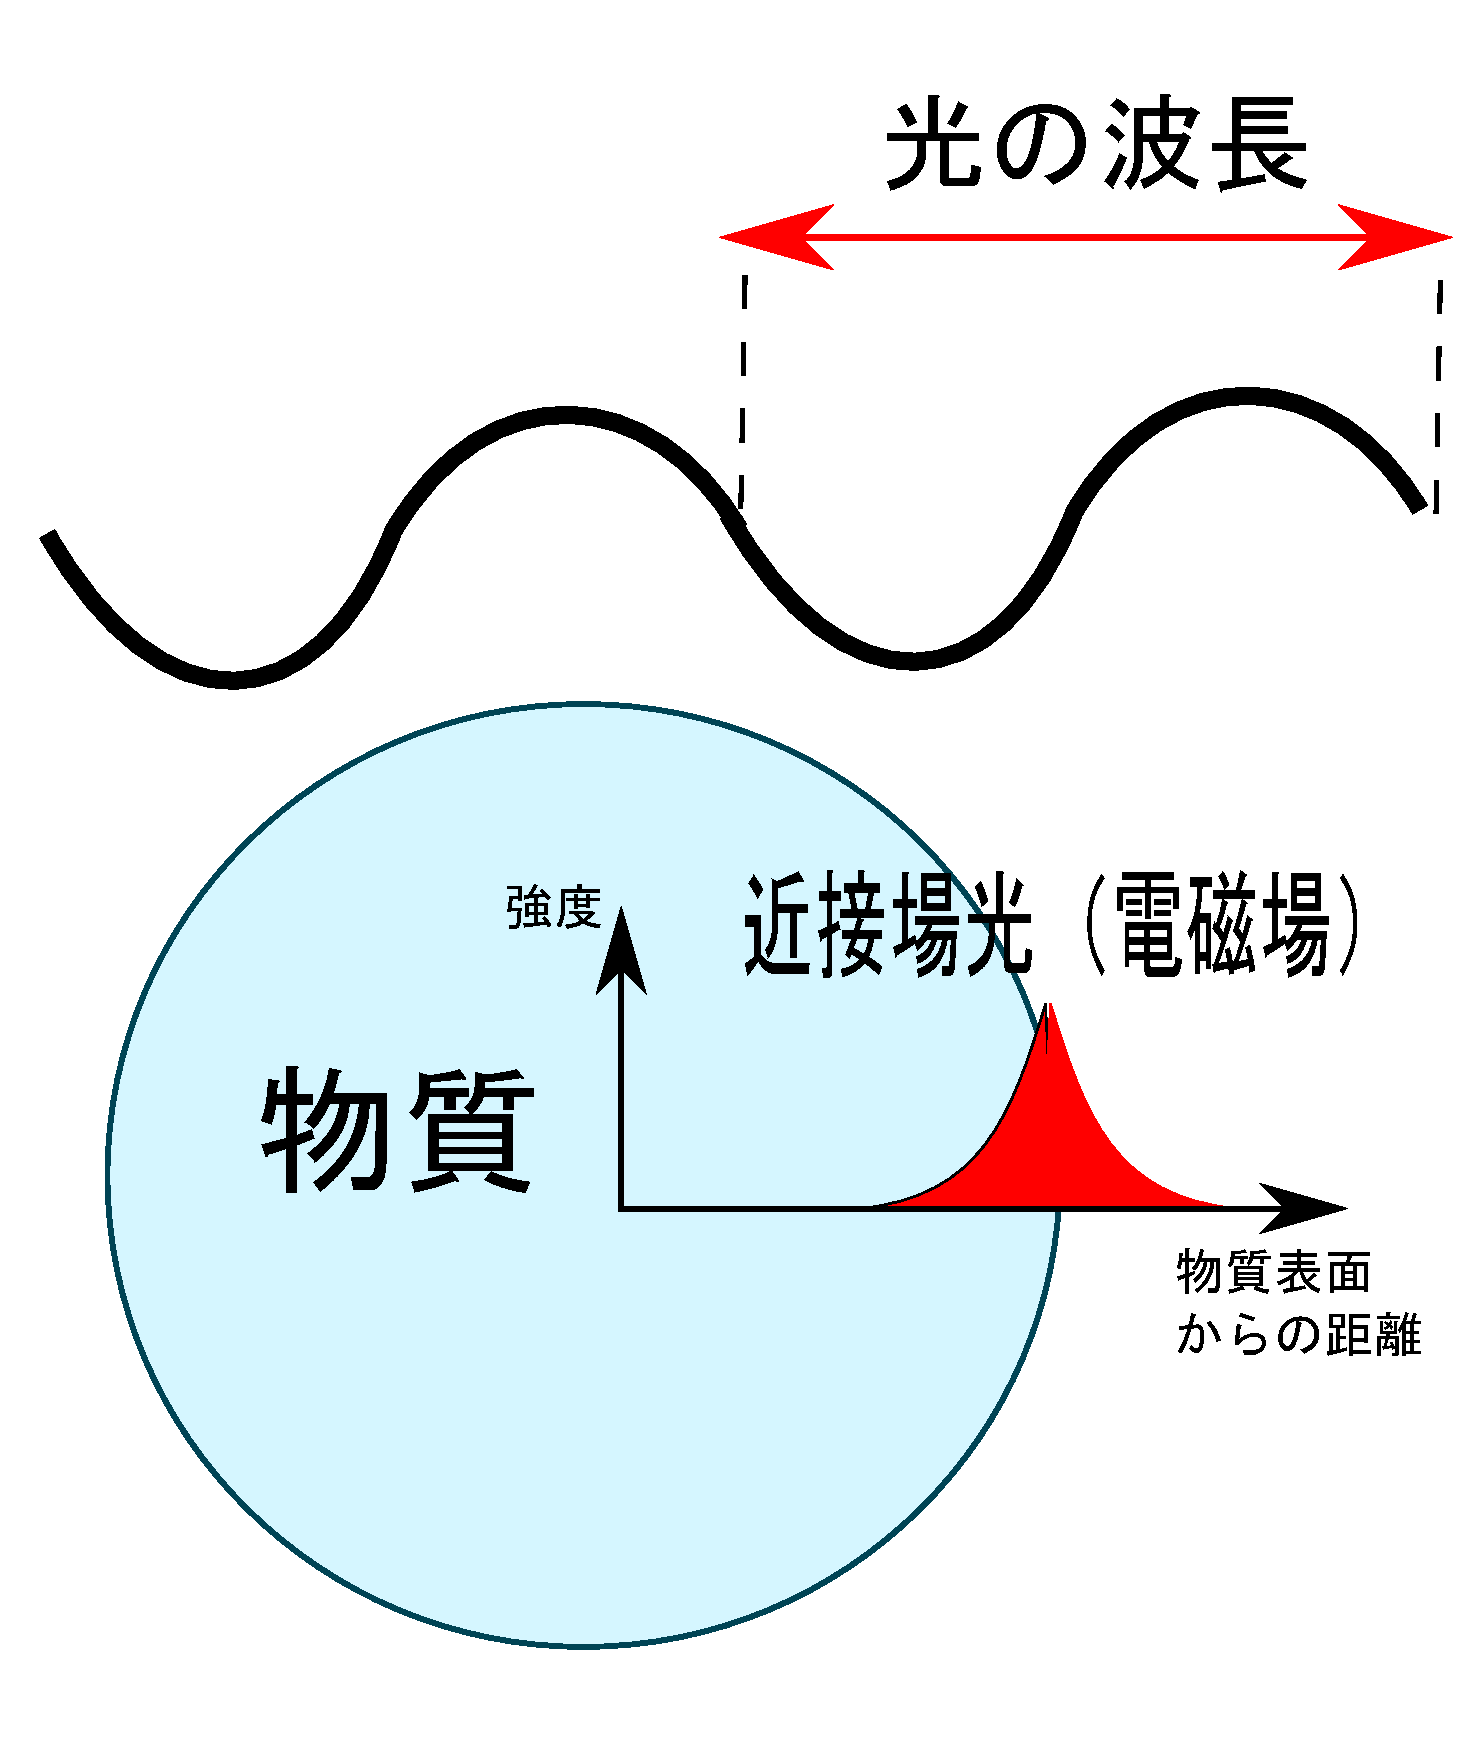
\includegraphics[keepaspectratio,scale=0.3]{fig/3/kinsetu.pdf}
\caption{近接場光}
\label{fig:kinsetu}
\end{center}
\end{figure}
\begin{figure}[t!]
\begin{center}
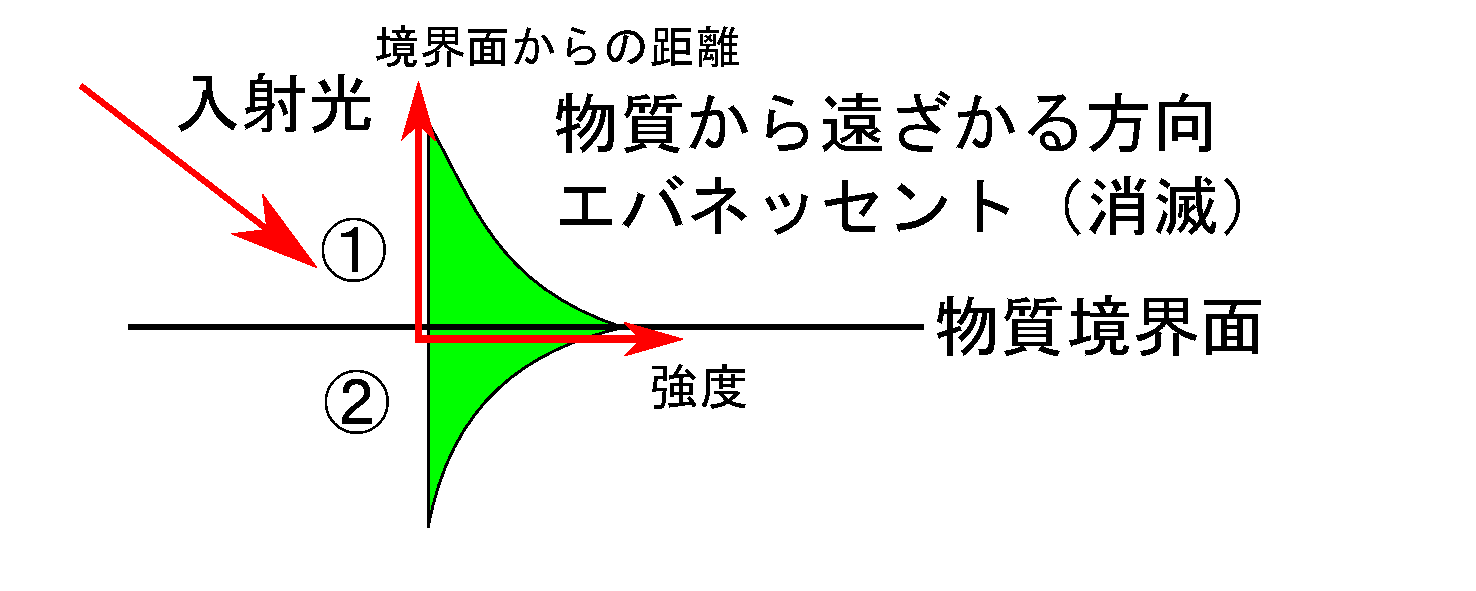
\includegraphics[keepaspectratio,scale=0.4]{fig/3/evanesent2.pdf}
\caption{エバネッセント光}
\label{fig:eva2}
\end{center}
\end{figure}
従来の光通信で広く使われている光素子の素材はガラスである.
これを半導体微細加工技術を用いて,半導体へと置き換える.
この技術によって半導体内を光が伝送できる.
ガラスから半導体へと素材を変えただけでは,光素子のゲート長のスケールは$cmからmm$のサイズに小さくなる.
これを$ \mu m$のスケールにするためには,半導体などのナノ加工技術がベースとしてある.
半導体のナノ加工技術が素子の加工技術のベースになり,近接場光の局在性をはじめとする近接場光にしかない特徴を活かして,
光信号をナノレベルで制御することが可能になって成り立つ技術がナノフォトニクスである.

\subsection{光デバイスとRace Logic}
前述した通り,光デバイスとは光伝搬信号を取り扱う素子を指す.
光伝搬信号の情報媒体は信号強度や位相,遅延時間といったアナログ量であり,
光伝搬信号はアナログ信号である.
電気デバイスであるCMOSトランジスタは電気信号を取り扱い,
その電気信号はデジタル信号である.
扱う信号がデジタル信号であるかアナログ信号であるかは二つのデバイスの大きな違いである.

また,Race Logicは動的計画法で解くことができる最適化問題の答えを
遅延時間というアナログ量で表現するアプローチである.

本研究では,情報媒体にアナログ量を取り扱う光デバイスと
Race Logicとの親和性に着目した.
ナノフォトニクック・デバイスをはじめとする
光デバイスの光速での信号処理という特徴から,
CMOSデバイスを用いたRace Logic回路よりも性能において優位になると考え,
光Race Logic回路を提案する.

\section{提案回路}
ナノフォトニック・デバイスを用いたRace logic(以下,光Race Logic)回路のセル構造を考えていく.
図\ref{fig:lightracelogiccell}に光Race Logic回路のセルの概要を示す.
\begin{figure}[t!]
\begin{center}
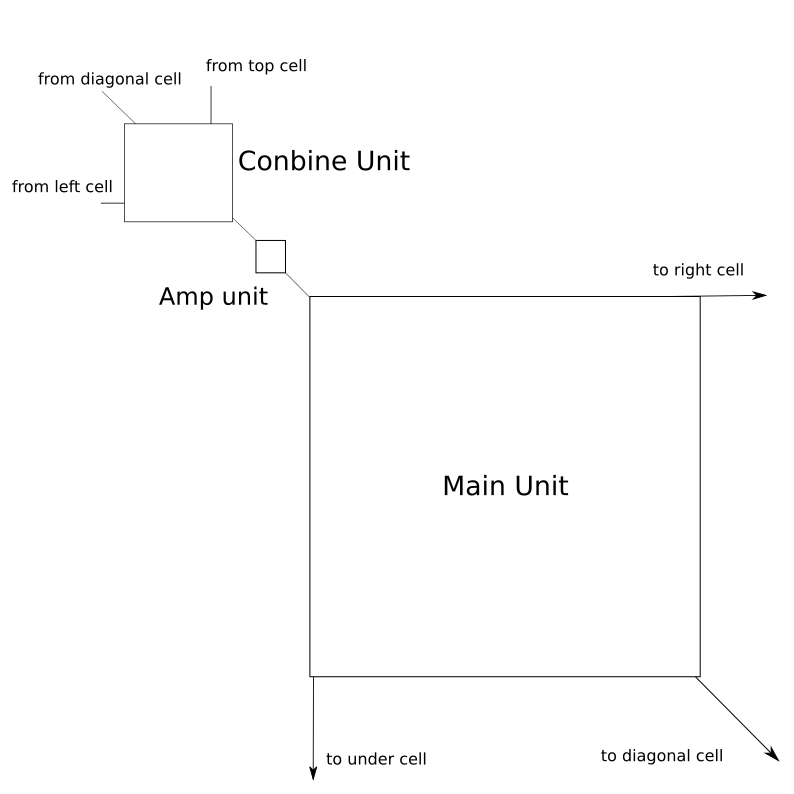
\includegraphics[keepaspectratio,scale=0.5]{fig/3/lightracelogic_cell_1.png}
\caption{光Race logic回路におけるセルの概要}
\label{fig:lightracelogiccell}
\end{center}
\end{figure}

セルは大きく分けて3つのユニットに分けて考えることができる.
まずは入力ユニットで,これは左・斜上・上のセルからの入力経路を持つ.
入力の次は合波ユニットで,ここは合波とそれに付随する処理を行うユニットである.
最長経路探索や最短経路探索,回路に設定する競争条件に合わせてその処理・構成が変わる.
その後,光伝搬信号はアンプユニットで光強度を増幅された後,メインユニット到達する.
メインユニットでは光伝搬信号の分波と任意の処理を施して,
光伝搬信号を次のセルへと出力する.
このユニットの構成と処理は回路に設定された競争条件によって変化する.
また,同期・非同期の処理に関しては合波ユニットもしくはメインユニット,あるいはその両方の構成で設定する.
対象とするアプリケーションや設定する競争条件によって,光Race Logic回路の構成は詳細に決定する.

今回はDNAのグローバル配列アラインメントスコア計算を対象とした
非同期型光Race Logic回路のarrayを提案する.
今回の提案回路で非同期型の構成を選択したのは,
光伝搬信号は蓄積が困難であるという点を考慮した結果である.
計算に用いるスコアマトリクスは式\ref{eq:mchun}を用いて求めた.
そのスコアマトリクスを図\ref{fig:scorematrix_3}に示す.
最下行と最右列はギャップスコアを表している.
\begin{figure}[t!]
\begin{center}
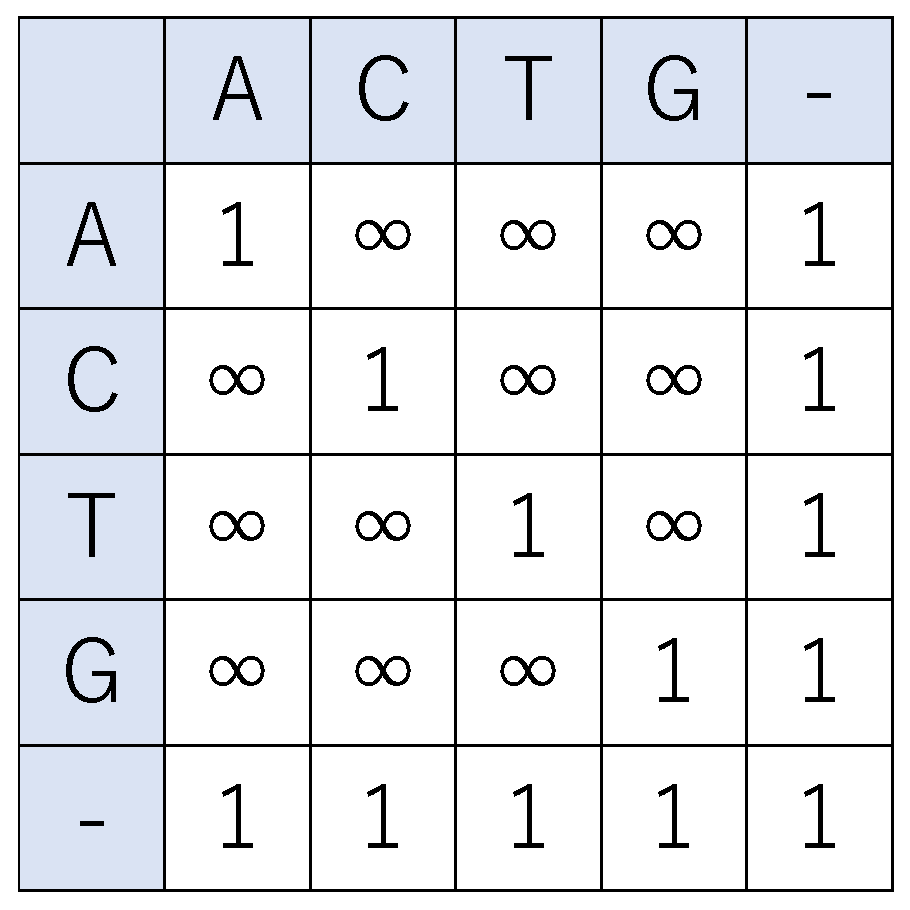
\includegraphics[keepaspectratio,scale=0.3]{fig/3/scorematrix.eps}
\caption{使用するスコアマトリクス}
\label{fig:scorematrix_3}
\end{center}
\end{figure}

図\ref{fig:proposalcell}に提案する回路のセル構造を示す.
\begin{figure}[t!]
\begin{center}
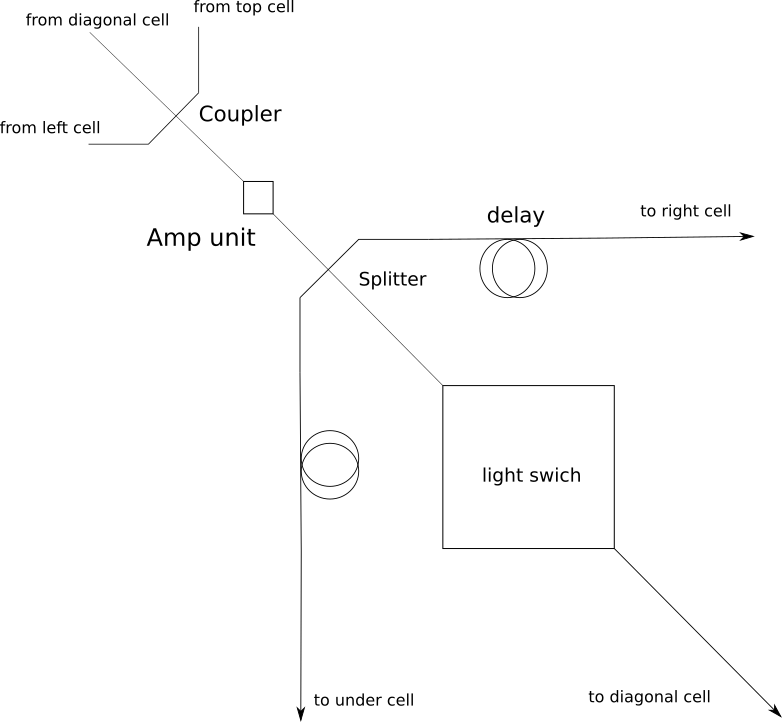
\includegraphics[keepaspectratio,scale=0.5]{fig/3/lightracelogic_cell_6.png}
\caption{提案回路のセル構造}
\label{fig:proposalcell}
\end{center}
\end{figure}
提案回路のセルにおいて,合波ユニットでは3入力1出力の光カプラを用いて合波が行われる.
この時,3方向から同時に光信号が入力された場合,
それぞれの光入力信号が光カプラに到達するまでの時間が同じになるよう調整する必要がある.
メインユニットでは1入力3出力の光カプラを用いて右,下,斜め下へに分波され,
各伝搬経路ごとにスコアマトリクスに基づいての重み付けがされている.
斜め下への伝搬経路では,光スイッチを通過し次のセルへと出力されるまでの遅延時間を
スコアマトリクスにおける一致スコアの1の重みを表す量として取り扱う.
この光スイッチでは,比較する文字列が一致した場合ON,
不一致の場合にOFFになるように設定する.
光スイッチがOFFの時,光伝搬信号は斜め下のセルに伝搬されない.
これは無限大の遅延時間を付加された,と考えることができ,不一致スコアに対応した重
み付けがされたとみなすことができる.
右,下への伝搬経路ではギャップスコアに基づく遅延が発生するように,
光遅延素子を設定する.
今回使用するスコアマトリクスにおいては,ギャップスコアは1の重みである.
これは一致スコアと同じ重みである.
よって今回,光遅延素子で設定すべき遅延時間は,
光遅延素子を通過して次のセルへ出力されるまでの遅延時間が
斜め下への伝搬経路で発生する遅延時間と同じになるような量である.

このセルを並べることでDNA配列アラインメントスコア計算を対象とした光Race Logic回路のarrayを構築する.
アレイに信号を入力してから出力されるまでの伝搬遅延が2つの文字列間の最適なアラインメントスコアに対応している.

この提案回路について,次章で検証・評価を行う.
